Small recap considering both cases in which we consider both following cases: the features are on the horizontal axes and the vertical one.
\setlength{\columnseprule}{0.4pt}
\begin{multicols}{2}
    \[
        X \in \mathbb{R}^{n \times p} \hspace{0.2cm} \text{centered and } \begin{cases}
        n & \text{ \# of samples}\\
        p & \text{ \# of features}
    \end{cases}
    \]
    \[
        C = \dfrac{1}{n-1}X^\intercal X (spd)    
    \]
    can be factorized:
    \[
        C = V\Lambda V^\intercal    
    \]
    The columns of $V$ are the eigenvectors of $C$ and $\Lambda$ is a diagonal matrix with the eigenvalues of $C$. The eigenvectors are also called \textbf{principal directions}. The \textbf{principal components} instead, are obtained as:
    \[
        XV    
    \]
    And they represent the coordinates of the original samples in the new basis. If we write $X = U\Sigma V^\intercal$ then
    \[
        \begin{split}
            C &= \dfrac{1}{n-1}V\Sigma^\intercal U^\intercal U\Sigma V^\intercal \\
            &= \dfrac{1}{n-1}V\Sigma^2 V^\intercal \\
        \end{split}    
    \]
    And we have also that:
    \[
        \lambda_i = \dfrac{1}{n-1}\sigma_i^2    
    \]
    Moreover, with SVD:
    \[
        XV = U\Sigma V^\intercal V = U\Sigma    
    \]
    Are still principal components.
    \newcolumn
    \[
        X \in \mathbb{R}^{p \times n} \hspace{0.2cm} \text{centered and } \begin{cases}
        n & \text{ \# of samples}\\
        p & \text{ \# of features}
    \end{cases}
    \]
    Now, in this case we simply need to interchange the roles for $U$ and $V$.
    \[
        C = \dfrac{1}{n-1}XX^\intercal = \dfrac{1}{n-1}U\Sigma^2 V^\intercal
    \]
    The principal directions are in $U$ (and indeed not in $V$ this time). To get the principal components we have to:
    \[
        X^\intercal U    
    \]
\end{multicols}
In Ridge we have found that:
\[
\underline{\hat{w}}_{R} = \arg \min_{\underline{w}} ||\underline{y} - \Phi\underline{w}||_2^2 + \lambda ||\underline{w}||_2^2
\]
Let's consider a binary classification problem so we have ($\underline{x}_i, y_i$) and $y_i \in \{-1, 1\}, \underline{x}_i \in \mathbb{R}^p$. Now consider Least squares for this problem:
\[
    \underline{\hat{w}}_{LS} = \arg \min_{\underline{w}} \sum_{i=1}^n (y_i - \underline{x}_i^\intercal \underline{w})^2 = \arg \min_{\underline{w}} \sum_{i=1}^n (1 - y_i\underline{x}_i^\intercal \underline{w})^2    
\]
You can easily check that the last equality holds in both values of $y_i$ because the parenthesis is squared.
There is an example on the notes that shows how the least squares is not a good idea for classification problems. Here are different loss functions we could use:
\begin{enumerate}
    \item Square loss: $L_i(y_i, \underline{X}_i^\intercal, \underline{w}) = (1 - y_i\underline{X}_i^\intercal \underline{w})^2$
    \item Ideal loss: $L_i(y_i, \underline{X}_i^\intercal, \underline{w}) = \begin{cases}
        0 & y_i\\
        1 & y_i\underline{X}_i^\intercal \underline{w} < 0\\
    \end{cases}$
    \item Hinge loss: $L_i(y_i\underline{X}_i^\intercal \underline{w}) = (1 - y_i\underline{X}_i^\intercal \underline{w})_{+}$
\end{enumerate}
Where $(a)_{+} = \begin{cases}
    a & \text{if } a > 0\\
    0 & \text{if } a \leq 0\\
\end{cases}$

Here is the plot of those functions:
\begin{center}
    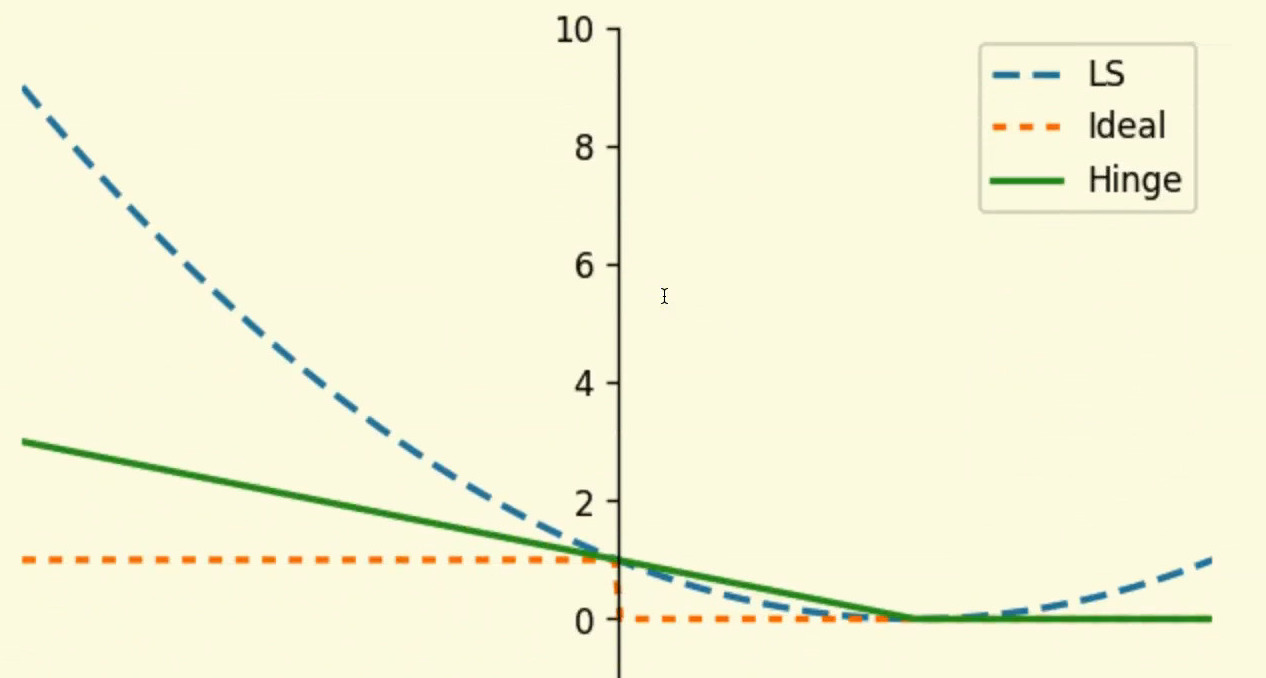
\includegraphics[]{../images/LossFunctions.jpg}
\end{center}
On the x axis you have $y_i\underline{X}_i^\intercal \underline{w}$. This picture can be divided in 3 points: if we are in the negative part (left part of the plot) this means that the predicted label is wrong and it has opposite sign with respect to the true label. In the middle part, the predicted label is correct but the margin is small. In the right part, the predicted label is correct and the margin is large. The square loss, differently from the other two, continue to grow even if the margin is large. The ideal loss is not differentiable and this is a problem for the optimization. The hinge loss is differentiable and it is the most used in practice. The ideal loss gives the same weight in the loss for a misclassified entry independently on our far is from the boundary. In the hinge instead the loss grows linearly with the distance and in the square grows squared. \\ 


\section{Computing derivatives}
Now we are going to consider different ways to compute the derivative of a function:
\begin{center}
    \begin{tabular}{|| m{14em} | m{12em} | m{20em} ||} 
     \hline
     Method & PRO & CONS \\ [0.5ex] 
     \hline\hline
     Manual computation & Exact, good for the proofs & Prone to error, expensive for complex functions\\ 
     \hline
     Numerical differentiation & Easy to program & Floating point precision*, computational cost\\
     \hline
     Symbolic differentiation & Exact, good for proofs &  Expression swelling**, not able to differentiate if conditions or loops  \\
     \hline
     Automatic differentiation (AD) & Exact, fast & Implementation \\
     \hline
    \end{tabular}
\end{center}

\noindent*: view jupyter notebook "Round\_off\&Truncation.ipynb" for more details.\\
**: big expressions of the derivative.\\

Consider this function:
\[
    y = f(x_1,x_2) = \sin((x_1 + x_2)x_2^2)     
\]
There are two possibilities for representing this function:
\begin{enumerate}
    \item \textbf{Wengert list} for a generic function $f: \mathbb{R}^n \to \mathbb{R}^m$ is defined as:
    \[
        \begin{cases}
            \text{Input variables: } v_{i-n} = x_i & i = 1, \dots, n\\
            \text{Intermediate variables: } v_i & i = 1, \dots, l\\
            \text{Output variables: } v_{n-i} = v_{l-i} & i = m-1, \dots, 0\\
        \end{cases}    
    \]
    Now, let's go back to out example function, in this case it's Wengert list formulation is the following:
    \begin{multicols}{2}
        \[
            \begin{split}
                v_{-1} &= x_1 = 1\\
                v_0 &= x_2 = 2\\
                \hline
                v_1 &= x_1 + x_2 = 3\\
                v_2 &= x_2^2 = 4\\
                v_3 &= v_1v_2 = 12\\
                v_4 &= \sin(v_3) = 0.536\\
                \hline 
                y &= v_4
            \end{split}    
        \]
        Notice that i've separated with the horizontal lines the different variables of the list. The input variables values have been chosen randomly just to compute the example with numbers.
    \end{multicols}
    How can we use the Wengert list for computing the derivative of a function? Let's consider the derivative of $y$ with respect to $x_1$:
    \[
        \begin{split}
            \dot{v}_{-1} &= \dot{x}_1 = 1\\
            \dot{v}_0 &= \dot{x}_2 = 0\\
            \hline
            \dot{v}_1 &= \dot{x}_1 + \dot{x}_2 = 1\\
            \dot{v}_2 &= 0\\
            \dot{v}_3 &= \dot{v}_1v_2 + v_1\dot{v}_2 = 4\\
            \dot{v}_4 &= \cos(v_3)\dot{v}_3 = 3.37\\
            \hline
            \dot{y} &= \dot{v}_4 = 3.37
        \end{split}     
    \]
    In this way we have splitted and computed only easy operations. This is called the \textbf{Forward Mode of Automatic Differentiation (AD)}. AD gives you the derivative computed for a certain popint. If we change points the opereations have to be done again.
    \item \textbf{Direct Acyclic Graph (DAG)}\\
    \begin{multicols}{2}
        \begin{tikzpicture}[
            SIR/.style={draw=red!60, fill=red!5, very thick, minimum size=5mm},
            node distance=2cm
            ]
            %Nodes
            \node[SIR]    (1)                    {$y = \sin(v_3)$};
            \node[SIR]    (2)       [below=of 1] {$v_3 = v_1v_2$};
            \node[SIR]    (3)       [below=of 2] {$v_1 = x_1 + x_2$};
            \node[SIR]    (4)       [right=of 3] {$v_2 = x_2^2$};
            \node[SIR]    (5)       [below=of 3] {$x_1$};
            \node[SIR]    (6)       [below=of 4] {$x_2$};
            
            %Lines
           \draw[->, very thick] (2.north)  to node[left] {$\dfrac{\partial y}{\partial v_3} = \cos(v_3)$} (1.south);
           \draw[->, very thick] (3.north)  to node[left] {$\dfrac{\partial v_3}{\partial v_1} = v_2$} (2.south west);
            \draw[->, very thick] (4.north)  to node[above right] {$\dfrac{\partial v_3}{\partial v_2} = v_1$} (2.south east);
            \draw[->, very thick] (5.north)  to node[left] {$\dfrac{\partial v_1}{\partial x_1} = 1$} (3.south west);
            \draw[->, very thick] (6.north)  to node[left] {} (4.south);
            \draw[->, very thick] (6.north west)  to node[left] {$\dfrac{\partial v_1}{\partial x_2} = 1$} (3.south east);
           \end{tikzpicture}

           As you can see on the nodes there are the values of the variables and on the arrows there are the derivatives. The arrows are the partial derivatives of the function with respect to the variable of the node. \textbf{To compute the derivative of the function wrt a certain variable, you need to consider all paths that connect the top of the graph with the desider variable}. From $y$ to $x_1$ there is a single path so it's easy but if you consider $y$ and $x_2$ there are 2 possible paths, in this case you need to add them.

           This is the \textbf{Reverse or Backward Mode of Automatic Differentiation (AD)}. It is more efficient than the forward mode because it computes the derivative of all the variables at the same time. It is used in neural networks because the number of variables is much higher than the number of samples.
    \end{multicols}
\end{enumerate}